%#%#%#%#%#%# L1448N Paper %#%#%#%#%#%#%#%#
%#%# Nickalas Reynolds and John Tobin %#%#
%#%#%#%#%#%#%# July  2017 %#%#%#%#%#%#%#%#

% SNOOPI For Perseus Region
%<http://almascience.nrao.edu/aq/?source_name_resolver=L1448N&result_view=observation&public_data=on&science_observations=on#sortCol=Release%20date&sortDir=asc&col_1=_checkbox_selector;;;&col_2=Source%20name;;;&col_3=Project%20code;;;&col_4=PI%20name;;;&col_5=Pub;;;&col_6=RA;;;&col_7=Dec;;;&col_8=Band;;;&col_9=Release%20date;;;&col_10=Observation%20date;;;&col_11=Velocity%20resolution;;;&col_12=Frequency%20support;;;&col_13=Angular%20resolution;;;&col_14=Continuum%20sensitivity;;;&col_15=Line%20sensitivity%20(10%20km%2Fs);;;>

%# document %#
\documentclass[preprint,12pt]{aastex62}
\usepackage{float}
%

%# New commands %#
% molecules
\newcommand{\htcn}{H$^{13}$CN}
\newcommand{\nthp}{N$_2$H$+$}
\newcommand{\ntdp}{N$_2$D$+$}
\newcommand{\cso}{C$^{17}$O}
\newcommand{\ceo}{C$^{18}$O}
\newcommand{\htcop}{H$^{13}$CO$^+$}
\newcommand{\co}{$^{12}$CO}
\newcommand{\sio}{SiO}
\newcommand{\lco}{\co\space      (J = 3$\rightarrow$2)}   % 346.~GHz
\newcommand{\lhtcn}{\htcn\space   (J = 4$\rightarrow$3)}   % 345.339756
\newcommand{\lcso}{\cso\space    (J = 3$\rightarrow$2)}   % 337.061104
\newcommand{\lhtcop}{\htcop\space (J = 4$\rightarrow$3)}   % 346.998347
\newcommand{\lsio}{\sio\space    (J = 7$\rightarrow$6)}   % 347.000031
%                 Continuum                     % 335.5
% misc
\renewcommand{\arcsec}{$^{\prime\prime}$}
\renewcommand{\arcmin}{$^{\prime}$}
\renewcommand{\deg}{$^{o}$}
\renewcommand{\micron}{$\mu$m}

\newcommand{\ab}{$\sim$}
\newcommand{\source}{L1448 IRS3B}
\newcommand{\sources}{L1448 IRS3A\&B}
\newcommand{\ra}{03$^{h}$25$^{m}$36.381$^{s}$}
\newcommand{\dec}{30\deg45\arcmin14\farcs710}
\newcommand{\radec}{RA = \ra, DEC = \dec}
\newcommand{\solm}{M$_{\odot}$}
\newcommand{\x}{$\times$}

% beam sizes
\newcommand{\csobeam}{0\farcs21$\times$0\farcs13} % check this !!!!!!
\newcommand{\siobeam}{0\farcs85$\times$0\farcs52}
\newcommand{\cobeam}{0\farcs19$\times$0\farcs11}
\newcommand{\htcopbeam}{0\farcs21$\times$0\farcs13}
\newcommand{\htcnbeam}{0\farcs21$\times$0\farcs13}
\newcommand{\contbeam}{0\farcs11$\times$0\farcs05}
\newcommand{\contbeamhigh}{0\farcs08$\times$0\farcs05}

%--------------------------------------------------------------------------------------%
%# beginning document %#
%--------------------------------------------------------------------------------------%
\begin{document}
\nocite{*}
%#%#%#%#%#%#%#%#%#%#%#%#%#%#%#%#%#%#%#%#%#%#%#%#%#%#%#
%# authors %#
%#%#%#%#%#%#%#%#%#%#%#%#%#%#%#%#%#%#%#%#%#%#%#%#%#%#%#
% author
\title{Kinematic Analysis of a Gravitationally Unstable Disk: L1448 IRS3B}
\shorttitle{L1448 IRS3B}
\shortauthors{Reynolds et al. (2018)}

\author{
Nickalas K. Reynolds\altaffilmark{1},John J. Tobin\altaffilmark{2},Patrick Sheehan\altaffilmark{2},Claire J. Chandler\altaffilmark{2},Leslie W. Looney\altaffilmark{3},Zhi-Yun Li\altaffilmark{4},Sarah I. Sadavoy\altaffilmark{5},Michael M. Dunham\altaffilmark{6,7},Dominique Segura-Cox\altaffilmark{8},Kaitlin Kratter\altaffilmark{9},Carl Melis\altaffilmark{10},Robert J. Harris\altaffilmark{11},Laura P\^erez\altaffilmark{12}\\\textit{Affiliations included after references}
}

\altaffiltext{1}{Homer L. Dodge Department of Physics and Astronomy, University of Oklahoma, 440 W. Brooks Street, Norman, OK 73019, USA}
\altaffiltext{2}{National Radio Astronomy Observatory, P.O. Box O, Socorro, NM 87801}
\altaffiltext{3}{Department of Astronomy, University of Illinois, Urbana, IL 61801}
\author{}
\altaffiltext{4}{Department of Astronomy, University of Virginia, Charlottesville, VA 22903}
\altaffiltext{5}{Harvard-Smithsonian Center for Astrophysics, 60 Garden St, MS 78, Cambridge, MA 02138}
\altaffiltext{6}{Department of Physics, State University of New York Fredonia, Fredonia, New York 14063, USA}
\altaffiltext{7}{Harvard-Smithsonian Center for Astrophysics, 60 Garden St, MS 78, Cambridge, MA 02138}
\altaffiltext{8}{Department of Astronomy, University of Illinois, Urbana, IL 61801}
\altaffiltext{9}{University of Arizona, Steward Observatory, Tucson, AZ 85721}
\altaffiltext{10}{Center for Astrophysics and Space Sciences, University of California, San Diego, CA 92093}
\altaffiltext{11}{Department of Astronomy, University of Illinois, Urbana, IL 61801}
\altaffiltext{12}{Departamento de Astronom\'ia, Universidad de Chile, Camino El Observatorio 1515, Las Condes, Santiago, Chile}

%#%#%#%#%#%#%#%#%#%#%#%#%#%#%#%#%#%#%#%#%#%#%#%#%#%#%#
%#%# Abstract %#%#
%#%#%#%#%#%#%#%#%#%#%#%#%#%#%#%#%#%#%#%#%#%#%#%#%#%#%#
\begin{abstract}
We present ALMA observations towards a known compact ($<$500 AU separation) triple system, L1448 IRS3B, in Band 7 (879~\micron). We resolve spiral structures in dust continuum in the circum-multiple disk of IRS3B and detect the known wide (\ab2300 AU) companion, IRS3A, within these observations, also resolving possible spiral structure. Using dense gas tracers, \lcso\space and \lhtcn\space, we resolve disk kinematics for both the circum-triple structure and the wide companion with high fidelity.  Further, we use the empirical PV-data and radiative transfer modeling of the molecular line emission to confirm that the disks are in Keplerian rotation with mass estimates of 1.1\solm\space for IRS3B and 1.4\solm\space for IRS3A. Through the continuum models, we estimate the mass of the fragmenting disk of IRS3B to be \ab0.64\solm, indicating this disk is massive enough to be gravitationally unstable. By analyzing the Toomre~Q, we find the IRS3B disk is consistent with a gravitationally unstable disk between the radii \ab100~AU to 600~AU. The embedded tertiary companion, IRS3B-c, is likely \ab0.09\solm. While Toomre~Q analysis of IRS3A, whose disk is measured to be \ab0.08\solm, indicates this source is gravitationally stable.
\end{abstract}


%#%#%#%#%#%#%#%#%#%#%#%#%#%#%#%#%#%#%#%#%#%#%#%#%#%#%#
%#%# Introduction %#%#
%#%#%#%#%#%#%#%#%#%#%#%#%#%#%#%#%#%#%#%#%#%#%#%#%#%#%#
\section{Introduction}
Star formation takes place in dense cores within molecular clouds \citep{1987ARAA..25...23S}, generally found within filamentary structures \citep{2014prpl.conf...27A}. The Perseus Molecular Cloud in particular hosts a plethora of young stellar objects (YSOs) and is nearby \citep[d\ab293 pc; e.g.][]{2018arXiv180803499O} making it an ideal target to study it's protostellar population \citep{2014ApJ...787L..18S,2009ApJ...692..973E}. By observing these YSOs during the first stages of star formation, we can learn about the early evolution of these cores into proto-planetary and/or proto-multiple systems \citep{2014prpl.conf..173L}.

Protostellar systems have been classified into several groups: Class 0, the youngest and most embedded objects characterized by low L$_{bol}$/L$_{submm}$, the less embedded but still dominated by their envelope Class I objects, and Class II objects which have shed their envelope and a protoplanetary disk forms. Most of stellar mass build-up is expected to occur during the Class 0 and Class I phase \citep[$<5\times$10$^{5}$yr; e.g.][]{2018arXiv180711262K,1987IAUS..115....1L} since by the time the system has evolved to Class II, most of the mass of the envelope has been either accreted or blown away by the outflows \citep{2006ApJ...646.1070A}. In order to fully understand star formation and multiple-star formation, it is important to target the youngest of the systems to characterize the initial conditions.

% work on this
% motivate how frequent multple systems are in field stars

\citet{2013ApJ...768..110C} presented a large (33 sources) survey towards known protostellar systems in nearby clouds (d$<$500 pc). This survey was conducted with the Submillimeter Array (SMA) 1.3~mm and 850~\micron\space dust continuum data. Their sample found 21 sources in binaries or higher-order multiplicities (separations \ag50-5000~AU) with a multiplicity frequency and companion fraction of 0.64 and 0.91 respectively. These frequencies were \ab2$\times$\space higher than those found for binary surveys towards Class I sources \citep[0.46 e.g.][]{2008AJ....135.2526C} and \ab4$\times$\space more frequent than surveys targeting main sequence stars \citep[0.21; e.g.][]{1991AA...248..485D} within the 50-5000~AU range. However, this survey suffered from poor spatial resolution, low sensitivity, and only targeted a subset of the known protostellar systems.

In order to better characterize protostellar multiplicity distributions, the VLA Nascent Disk and Multiplicity (VANDAM) survey \citep{2016ApJ...818...73T} targeted all known protostars down to 15 AU scales within the Perseus Molecular Cloud. They confirmed the high multiplicity fraction (MF) on 50-5000~AU scales of \citet{2013ApJ...768..110C} and surpassed them with superior spatial resolution and sensitivities finding the multiplicity fraction of Class 0 protostars \ab57\% (15-10,000~AU scales) and \ab25\% for close ($<$500~AU separation) companions. It was during this survey that L1448 IRS3B, a compact ($<$300~AU) triple system, was discovered. \citet{2016Natur.538..483T} observed this source at 1.3~mm, resolving the spiral arms, kinematic rotation signatures in \ceo, and strong outflows originating from the system.

% fix figure. Try with aplpy just make the triplet and wide aplpy calls without scales
\begin{figure}[H]
\begin{center}
% \includegraphics[width=0.75\textwidth]{img/poster_cont_all_clean.eps}
\includegraphics[width=\textwidth]{img/double_panel_horiz.eps}
\end{center}
\caption{\normalsize The high resolution 879~\micron\space observations of the triple protostellar system L1448 IRS3B and its wide companion IRS3A. The middle image zooms in on the triple structure. The inner binary (IRS3B) is separated by 75 AU and has a tight spiral circumbinary disk with the embedded source 230 AU away from the binary within one of the arms. The right image zooms in on IRS3A (d\ab2300AU), featuring possible spiral structure. The yellow boxes in the left image are location cuts for the two right images of \ab\x3 zoom-ins of the respective sources (middle and right for L1448 IRS3B and IRS3A, respectively). The beam size of each panel is shown in lower right (\contbeam\space using Briggs Robust parameter of 0.5).}\label{fig:contimage}
\end{figure}

L1448 IRS3B (Figure~\ref{fig:contimage}) has a hierarchical configuration, of which the inner binary (separation \ab0\farcs25 (75~AU), denoted -a and -b, respectively)) and the embedded tertiary (separation \ab0\farcs8 (240~AU), denoted -c). A wide (separation \ab 8\arcsec) companion, IRS3A, was also captured within these observations. \citet{2016ApJ...818...73T}\space found evidence for Keplerian rotation and found that the circumtriple disk was likely gravitationally unstable. It is believed there exists three main pathways for forming multiple systems: turbulent fragmentation \citep[1000s of AU; e.g.][]{1989ApJ...347..959A,2010ApJ...708.1585K,2012MNRAS.419.3115B}, thermal fragmentation \citep[1000s of AU; e.g.][]{2013ApJ...764..136B}, and/or gravitational instabilities \citep[100s of AU; e.g.][]{2011MNRAS.410..559M,2009MNRAS.392..413S}.

Here we detail our follow-up observations of L1448 IRS3B with the Atacama Large Millimeter/Submillimeter Array (ALMA), with high resolution and sensitivity. We use kinematic tracers to characterize rotation within the disks of IRS3B and IRS3A. We show our observations and data reduction techniques within Section~\ref{sec:obs}, we discuss our empirical results in Section~\ref{sec:results}, further detail our models and the results produced in Section~\ref{sec:modelresults}, and finally we detail implications of our empirical and model results and discuss future endeavors. 

%#%#%#%#%#%#%#%#%#%#%#%#%#%#%#%#%#%#%#%#%#%#%#%#%#%#%#
%#%# Observations %#%#
%#%#%#%#%#%#%#%#%#%#%#%#%#%#%#%#%#%#%#%#%#%#%#%#%#%#%#

\section{Observations}\label{sec:obs}
The ALMA located in Chile, observed \source\space(\radec) in Band 7 (879~\micron) during Cycle 4.
The target was to be observed during two configurations, a long (C40-6) and a compact (C40-3) baseline configuration in order to fully recover the total flux out to \ab5\arcsec\space in addition to resolving the source.

The extended configuration, C40-6, was used on 2016 October 1\&4 with 45 antennas. The baselines sampled span 15 to 3200 (0\farcs05\space agnular resolution to 5\arcsec) for a total of 4495 seconds on source (8052 seconds total). While the compact configuration, C40-3, was observed on 19 December 2016 with 41 antennas. The baselines sampled spanned 15 to 490 meters (0\farcs4 angular resolution to 5\arcsec largest angular scales) for a total of 1335 seconds on source (3098 seconds total).


The correlator was configured to observe \lco, \lcso, \lhtcop, \lhtcn, \lsio, and a broad 2~GHz continuum band centered at 335.5~GHz (894~\micron). A summary of the correlator setup is provided in Table 1. The complex gain calibrator was J0336$+$3218, the bandpass calibrator was J0237$+$2848, and the flux calibrator was the quasar J0238$+$1636. 

The raw data were reduced using the Cycle 4 ALMA pipeline using CASA \citep{2007ASPC..376..127M} version 4.7.0. We thoroughly inspected the data and verified the high fidelity. All further processing was done using the CASA 4.7.2 and the reduction sequence is described here. To maximize the sensitivity of the continuum observations, emission free channels from the molecular line spectral windows were added to the continuum after appropriate flagging and splitting of the emission regions was performed. The total bandwidth recovered from this method was \ab1.2~GHz in conjunction with the continuum spectral window bandwidth of 1.875~GHz, yields \ab3~GHz of continuum bandwidth. The observations achieved 0.069~mJy continuum sensitivity, 4~mJy/channel for \co, 3.7~mJy/channel for \cso, 4.5~mJy/channel for \htcn, 4.5~mJy/channel for \htcop, and 0.5~mJy/channel for \sio.

Given the high signal-to-noise (S/N) of the source, we performed self-calibration on the data to further increase the S/N by correcting short timescale phase and amplitude fluctuations. The separate configuration data sets were then concatenated using the task \textit{concat}. The resulting images were generated from this concatenated dataset using Briggs Weighting Robust parameter of 0.5. The beamsize of the continuum image is \contbeam\space (\ab32$\times$15~AU) and \cso\space beamsize is \csobeam\space (\ab79$\times$50~AU). 

During the high-resolution execution, an error was made when determining the correlator setup for SiO. The central frequency of the spectral window was adjusted to a lower value (from \ab347.27~GHz to \ab347.01~GHz), outside of the frequency range for SiO. The resulting spectral window was not centered over any visible emission lines; however, the window was fully used for the continuum multi-frequency analysis since no emission lines were discernable. 
    
\begin{deluxetable}{cccccccc}
\tablewidth{0pt}
%\rotate
\tabletypesize{\scriptsize}
\tablecaption{Summary of Observations}
\tablehead{
  \colhead{Source} & \colhead{RA}      & \colhead{Dec}      &\colhead{Config.\tablenotemark{a}}  & \colhead{Resolution} &\colhead{LAS\tablenotemark{b}} & \colhead{Date} & \colhead{Calibrators}\\
                   & \colhead{(J2000)} &  \colhead{(J2000)} &                   &                      &              & \colhead{(UT)} &   \colhead{(Gain, Bandpass, Flux)} \\
}
\startdata
L1448 IRS3B        & 03:25:36.382 & 30:45:14.715 & C40-6 & 0\farcs12 & 1\farcs3  & 1 and 4 October 2016 & J0336$+$3218,J0237$+$2848,J0238$+$1636    \\
L1448 IRS3B        & 03:25:36.382 & 30:45:14.715 & C40-3 & 0\farcs59 & 5\farcs6 & 19 December 2016     &  J0336$+$3218,J0237$+$2848,J0238$+$1636 \\
\enddata
\tablenotetext{a}{C40-6 - Extended and C40-3 - Compact} 
\tablenotetext{b}{LAS- Largest Angular Scale} 
\end{deluxetable}\label{table:obssummary1}

% split all these to two pannels. Low velocity and high velocity
\begin{figure}[H]
\begin{center}
   \includegraphics[width=0.8\textwidth]{img/L1448IRS3B_C17O_image_taper1500k__splitMoments.eps} % c17o
\end{center}
   \caption{ \cso\space tracing the rotating gas within the disk. In tandem with the continuum images, this gas provides insight into the kinematics of the gaseous circumstellar disks. Contours start at 7(7)$\sigma$ and iterate by 5(5)$\sigma$ for the red(blue) respectively. The $\sigma$~level is 2.9~mJy. The beam size is \csobeam.The velocity ranges are: 1.2$\rightarrow$3, 3$\rightarrow$4.8,4.8$\rightarrow$6.2, 6.2$\rightarrow$7.7~km/s for the respective high-velocity blue, low-velocity blue, low-velocity red, and high-velocity red doppler shifted emission.}\label{fig:c17omoment}
\end{figure}
\begin{figure}[H]
\begin{center}
   \includegraphics[width=0.8\textwidth]{img/L1448IRS3B_H13COp_image_taper1500k_.image.integratedb.eps} % h13co+
\end{center}
   \caption{\htcop\space tracing the less dense gas of the disk. This line is tracing the intermediary gaseous material between the outer disk and the envelope. Contours start at 6(6)$\sigma$ and iterate by 8(8)$\sigma$ for the red(blue). The $\sigma$~level is 2.4~mJy. The beam size is \csobeam.The velocity ranges are: 2.3$\rightarrow$4.1 and 5$\rightarrow$6.8~km/s for the respective blue and red doppler shifted emission.
   }\label{fig:h13copmoment}
\end{figure}
\begin{figure}[H]
\begin{center}
   \includegraphics[width=0.49\textwidth]{img/L1448IRS3B_H13CN_clean_image_2_binned__totalMoments_irs3a.eps} % h13cn
   \includegraphics[width=0.49\textwidth]{img/L1448IRS3B_H13CN_clean_image_2_binned__binnedMoments.eps} % h13cn
\end{center}
   \caption{ \htcn\space. The left image shows IRS3A, which the gas is more closely tracing the kinematics of the inner disk with extended structure outside the disk. However, for the right image, IRS3B, this line appears to coincide with the launch location of the outflow from the tertiary, IRS3B-c. Contours start at 3(3)$\sigma$ and iterate by 3(5)$\sigma$ for the red(blue). The $\sigma$~level is 1.6~mJy. The beam size is \csobeam. The velocity ranges for IRS3A are: 1.6$\rightarrow$4.8, 5.2$\rightarrow$11.2~km,4.8$\rightarrow$6.2, 6.2$\rightarrow$7.7~km/s for the respective blue and red doppler shifted emission. The velocity ranges for IRS3B are: 1.6$\rightarrow$3.8, 3.8$\rightarrow$4.8,5.2$\rightarrow$7.8, 7.8$\rightarrow$11.2~km/s for the respective high-velocity blue, low-velocity blue, low-velocity red, and high-velocity red doppler shifted emission.
   }\label{fig:h13cnmoment}
\end{figure}

%#%#%#%#%#%#%#%#%#%#%#%#%#%#%#%#%#%#%#%#%#%#%#%#%#%#%#
%#%# Results %#%#
%#%#%#%#%#%#%#%#%#%#%#%#%#%#%#%#%#%#%#%#%#%#%#%#%#%#%#
\section{Results}\label{sec:results}

%#%#%#%#%#%#%#%#%#%#%#%#%#%#%#%#%#%#%#%#%#%#%#%#%#%#%#
%#%# Stellar Mass %#%#
%#%#%#%#%#%#%#%#%#%#%#%#%#%#%#%#%#%#%#%#%#%#%#%#%#%#%#
\subsection{Kinematics}
% work on this section
\cso\space a less abundant isotopologue of \co, appears to trace the gas within the disk of IRS3B. This gas structure extends to further radii than the dust continuum, indicating a strong gas precense within the disk, as expected of this young system. This molecule is used as a proxy for the gaseous contribution in the disk if we assume ISM abundances of this molecule. \htcop\space (Figure~\ref{fig:h13copmoment}) appears to trace much larger scale emission surrounding the disk of IRS3B. This is indicative of emission from the inner envelope or the more diffuse outer protostellar disk. The last molecular line, \htcn\space (Figure~\ref{fig:h13cnmoment}) is tracing the more dense and energetic parts of the disks. For IRS3B, the molecule appears to trace an apparent outflow from the tertiary protostar. For IRS3A, the molecule is possibly tracing the kinematics of the inner disk due to the compactness of the emission near the protostar and the appearance within the disk place.

In order to analyze the kinematics of these sources, we first evaluate the sources using a Position-Velocity (PV) diagram which collapses the 3-D nature of the data cubes into a 2-D data image. This works by reducing the number of absolute spatial axes (RA and Dec) to a displacement axis while preserving the velocity axis of the data. This allows for an estimation of several parameters via examining the respective doppler shifted components. 

A secondary preliminary evaluation method is through a modified PV diagram, herein ``Peak PV'' diagram \citep{2018ApJ...856..164T} which allows for a direct comparison of the rotation curve against Keplerian rotation and/or conservation of angular momentum.

%#%#%#%#%#%#%#%#%#%#%#%#%#%#%#%#%#%#%#%#%#%#%#%#%#%#%#
%#%# Stellar Mass %#%#
%#%#%#%#%#%#%#%#%#%#%#%#%#%#%#%#%#%#%#%#%#%#%#%#%#%#%#
\subsubsection{Protostar Masses}
We show the integrated intensity (Moment 0) map of \cso\space in Figure \ref{fig:c17omoment} which is tracing the emission of the gaseous disk. With numerous methods, we estimate the mass of the gaseous disk and recover the protostellar mass limit. We first determine the protostellar mass by analyzing the Position Velocity (PV) diagram of the channel maps to determine regions indicative of Keplerian rotation.

% work on this
%and second to model the visibilities and generate a Keplerian model that best describes the emission.

For the L1448 IRS3B source, the gas tracer \cso\space was used and the resulting PV diagram is shown in Figure \ref{fig:l1448npv}. To generate the PV diagram, strips of position angle 210\deg\space were extracted and summed, each with a width of 105~pixels (\ab1\farcs55). The PV diagram velocity axis is centered on the system velocity of 4.75 km/s and spans 5 km/s on either side; while the position axis is centered just off of the inner binary, determined to be the kinematic center, and spans 5\arcsec (\ab1500~AU) on either side. The kinematic center was determined via the highest velocity emission channels. The dotted while lines trace the Keplerian rotation curve ($V(R) = \sqrt(GM/R)$) of 1.1\solm which fully encapsulates the \cso\space emission from the source. This diagram provides a rough initial estimate of protostellar mass \citep[e.g.][]{2016MNRAS.459.1892S}.

For the L1448 IRS3A source, the dense gas tracer \htcn\space was used and is shown in Figure \ref{fig:l1448npv}. To generate the PV diagram, strips of position angle 90\deg\space were extracted and summed, each with a width of 51~pixels (\ab0\farcs88). We chose a different molecular line for IRS3A due to \cso\space being faint in this source. The velocity cut is centered on the system velocity of 5.4 km/s and spans 6.2 km/s on either side. The position cut is centered on the continuum source (coincides with kinematic center), and spans 3\arcsec (\ab880~AU) on either side. This provides a large enough window to collect all of the emission from the source. The dotted while lines detail the Keplerian model of 1.4\solm which reasonably well describes this source. 

While PV diagram fitting is not a rigorous way to characterize these sources, it provides reasonable estimates for the more rigorous modeling approach. From this analysis can constrain several system parameters to smaller regions of phase space: system velocity, kinematic center position, position angle, inclination, and stellar mass.

\begin{figure}[H]
\begin{center}
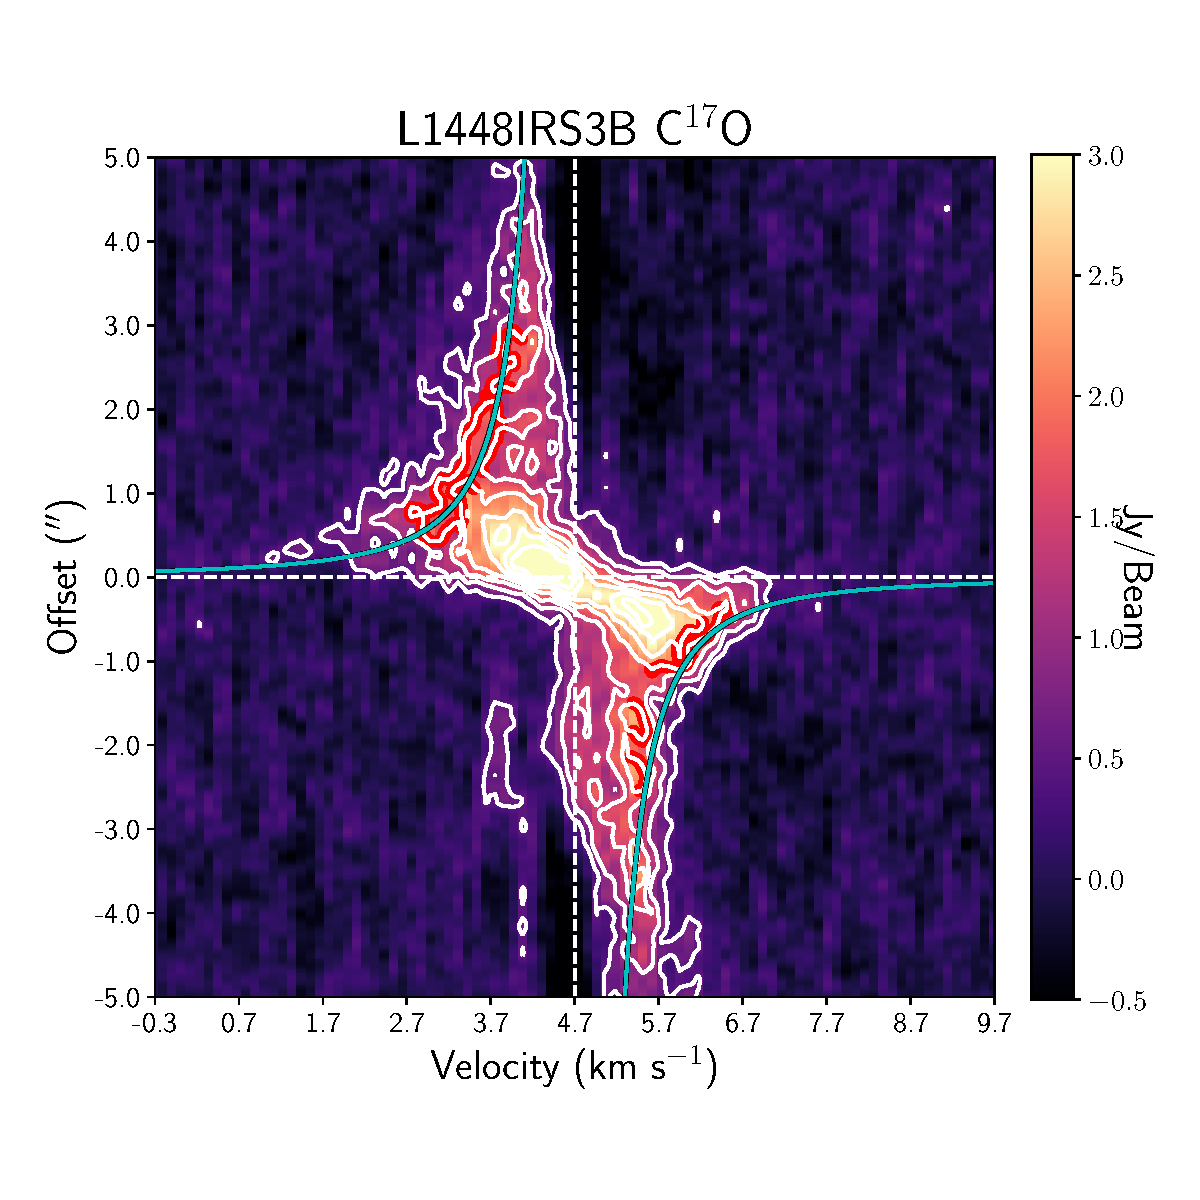
\includegraphics[width=0.44\textwidth]{img/irs3b_c17o_pv.eps}
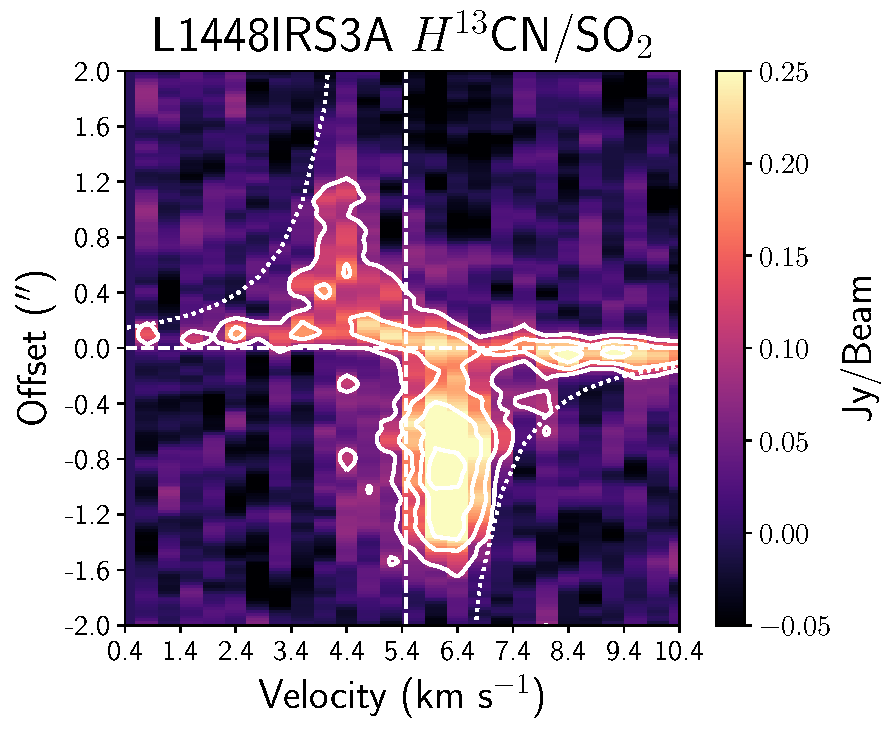
\includegraphics[width=0.44\textwidth]{img/irs3a_h13cn_pv.eps}
\end{center}
\caption{Position-Velocity Diagram \textbf{Left:} IRS3B \cso\space with the dotted lines corresponding to 1.1\solm. Demonstrating the data could be reproduced reasonably well with a Keplerian disk of roughly 1.1\solm. Position-Velocity Diagram \textbf{Right:} IRS3A \htcn\space with the dotted lines corresponding to 1.4\solm. Like-wise, this PV diagram places a constraint on the possible protostellar mass parameter of \ab1.4\solm. The IRS3A data is less well constrained due to the lower spatial sampling available due to the size of the source and its placement in the less sensitive regime of the primary beam.}\label{fig:l1448npv}
\end{figure}

%#%#%#%#%#%#%#%#%#%#%#%#%#%#%#%#%#%#%#%#%#%#%#%#%#%#%#
%#%# Rotation Analysis %#%#
%#%#%#%#%#%#%#%#%#%#%#%#%#%#%#%#%#%#%#%#%#%#%#%#%#%#%#
\subsection{Rotation Analysis}
To construct the Peak PV diagram, we fit the the peak intensity of each channel with a 2-D Gaussian to determine the central location of the emission. We plot these results of radius and velocity (relative to system velocity) in Figure~\ref{fig:peakpvc17o} in log-log space. With the points in log-log space we can simultaneously fit a power law function to the set to discern the underlying kinematics more easily. Keplerian rotation is indicated by a slope of \ab-0.5 (v$\propto$R$^{-0.5}$) while conservation of momentum is indicated by a slope of \ab-1 (v$\propto$R$^{-1}$) \citep{2013ApJ...772...22Y,2014ApJ...796..131O}. 

We analyze the \cso\space emission of IRS3B and identify the disk is well fit by a Keplerian rotation curve with a slope of $-0.5$\space and is indicative of a central mass of 1.1\solm.

\begin{figure}[H]
\begin{center}
\includegraphics[width=0.8\textwidth]{img/L1448IRS3B_c17o_peakPV.eps}
\end{center}
\caption{``Peak Position-Velocity'' Diagram of IRS3B \cso\space emission with the black line corresponding to the best fit. This demonstrates the compact ($<$150~AU) emission is well described with a Keplerian disk of roughly 1.1\solm. The gray points are excluded from the fit.}\label{fig:peakpvc17o}
\end{figure}
\begin{figure}[H]
\begin{center}
\includegraphics[width=0.8\textwidth]{img/L1448IRS3B_h13cop_peakPV.eps}
\end{center}
\caption{``Peak Position-Velocity'' Diagram of IRS3B \htcop\space emission with the black line corresponding to the best fit. This molecule is tracing a region outside the region described by \cso. This is indicative of it tracing an inner envelope or outer disk of IRS3B. The gray points are excluded from the fit.}\label{fig:peakpvh13cop}
\end{figure}


%#%#%#%#%#%#%#%#%#%#%#%#%#%#%#%#%#%#%#%#%#%#%#%#%#%#%#
%#%# Surface Density %#%#
%#%#%#%#%#%#%#%#%#%#%#%#%#%#%#%#%#%#%#%#%#%#%#%#%#%#%#
\subsubsection{Disk Mass}\label{sec:surfden}
The dust continuum observations can be used to estimate the the total mass of the disk surrounding IRS3B-ab and further, can be used to estimate the mass of the IRS3B-c, tertiary source, itself. The observations of the circumtriple disk, IRS3B, resolved the dust spiral structure, so to analyze the disk for its global properties rather than the local properties, we smooth the emission by tapering the UV-visibilities to 375~k$\lambda$. This method fully recovers the flux of the disk, but smoothes over the more detailed structure. If we make the assumption that the disk is isothermal, optically thin, and the dust and gas are well mixed, then we can derive the disk mass from the simple equation:

\begin{equation}
    M_{dust} = \frac{D^2 F_{\nu}}{\kappa_{\nu}B_{\nu}(T_{dust})}
\end{equation}

where D is the distance to the region (293 pc), F$_{\nu}$\space is the flux density, $\kappa_{\nu}$\space is the dust opacity, B$_{\nu}$\space is the Planck function for a dust temperature, and T$_{dust}$\space is taken to be the temperature of a typical protostar disk at a given radius from the protostar. The $\kappa_{\lambda}$\space at $\lambda$ = 1.3~mm was adopted from dust opacity models and previous studies with the limits between 0.899 cm$^2$g$^{-1}$, typical of dense cores \citep{1994AA...291..943O}. We then appropriately scale the opacities via the equation:

\begin{equation}
    \kappa_{879~\mu m} = \kappa_{1.3}\times\frac{1.3~mm}{879~\mu m}^{\beta}
\end{equation}

assuming the index $\beta$\ab1.7 as indicative of younger, more embedded cores \citep{1994AA...291..943O}.

If we assume the canonical ISM gas-to-dust mass ratio of 100:1 \citep{1978ApJ...224..132B}, we estimate the total mass of the IRS3B-ab disk to be 0.65\solm\space for $\kappa\approx$\space 0.899 cm$^2$g$^{-1}$. While the dust to gas ratio may be evolving in the disk at various regimes, we adopt a constant value \citep{2014ApJ...788...59W}. Of this total mass, we estimate 0.09\solm to be associated with the IRS3B-c, the embedded tertiary source. Note, we adopted a T$_{dust}$ = 45~K since the peak brightness temperature of the source is \ab23~K. This was determined by fitting a 2-D Gaussian region around the tertiary using the built-in \textit{casa} 2D Fit Tool. The initial fit was restricted to a region defined by a circular aperture centered on the tertiary of size 0\farcs45$\times$0\farcs48. The 2D fit yielded a peak intensity of 190~mJy/beam within a region 0\farcs312$\times$0\farcs276. This high peak brightness is indicative of an optically thick region, so likely our mass estimate is a lower limit. We perform the same analysis towards the wide companion source and arrive at a disk mass estimate of 0.06\solm. The peak brightness temperature of the wide companion source is \ab10~K (peak intensity \ab66~mJy/beam within a 0\farcs536$\times$0\farcs244 aperture) so we adopted a T$_{dust}$ = 20~K. For all the above measurements, in constructing the power law temperature profile of the disk, we limit the lower bound for the temperature to be 20~K 

% 59.3* ( 1.222E3/ (341.0606)**2 / (.536*.244))

\subsubsection{Surface Density}

With the high spatial and spectral resolution, we constructed a annuli cut of the continuum and moment map zero (integrated intensity) of \cso. The apertures for the annuli cuts were defined by the area of the synthesized beam with radii spanning out to \ab3\arcsec\space to completely recover the emission. With this method we construct a radial surface density to analyze the stability of the disk (Figure~\ref{fig:toomreq})

In order to remove the effects of the disk asymmetries found in this source, we use the deprojected images, described in the appendix, of the source, fit using an inclination of 45\deg\space and a position angle of 28\deg. We deprojected the \textit{UV} coordinates and regenerated new images using the same methods outlined in Section~\ref{sec:obs}. With this deprojection, we can then directly compare the integrated emission found in each respective annulus versus the radius the emission is present. We can then simply divide the recovered flux density by the corresponding aperture area to recover a surface density brightness.

%#%#%#%#%#%#%#%#%#%#%#%#%#%#%#%#%#%#%#%#%#%#%#%#%#%#%#
%#%# Results %#%#
%#%#%#%#%#%#%#%#%#%#%#%#%#%#%#%#%#%#%#%#%#%#%#%#%#%#%#
%# Analysis, Disk Dust and Gas mass, Surface Density, PV Diagrams, Stability %#
%In this section we will detail our procedures for first estimates of protostellar parameters and then discuss the results of the more rigorous and robust models. The summary of these methods is provided in Table \ref{table:diskanmod}. 
%#%#%#%#%#%#%#%#%#%#%#%#%#%#%#%#%#%#%#%#%#%#%#%#%#%#%#
%#%# Model %#%#
%#%#%#%#%#%#%#%#%#%#%#%#%#%#%#%#%#%#%#%#%#%#%#%#%#%#%#
\section{Models}\label{sec:modelresults}
We utilize the methods described in \citet{2017ApJ...846L..26W} for the molecular line emission modeling and \citet{2017ApJ...851...45S} for the continuum modeling. We use RADMC-3D \citep{2012ascl.soft02015D} to perform the radiative transfer models and use GALARIO \citep{2018MNRAS.476.4527T} to generate the model visibilities. We simultaneously fit the visiblities and the SED by utilizing a Markov Chain Monte Carlo approach supported by Bayesian statistics to provide a robust and rigorous model of the observations for further analysis (\cite[emcee]{2013PASP..125..306F} and PDSPY\footnote{https://github.com/psheehan/pdspy.git}).

We generate a set of priors for the protostellar parameters based off of observational constraints of the system, these priors are then sampled via a normal distribution and fed into a Markov Chain Monte Carlo Affine Invariant Algorithm \citep[emcee]{2013PASP..125..306F} to generate the model parameters, these parameters are then used to construct radiative transfer models with RADMC-3D, which are subsequently cross-compared with the observed data in the UV-plane. The probability of the parameters for this comparison is then updated internally and the whole process is repeated until convergence.

RADMC-3D \citep{2012ascl.soft02015D} is a robust radiative transfer code written in Fortran 90 for modeling continuum radiative transfer through dusty media, however, extensive work has been done to allow for gas line transfer models to be implemented as well. This code provides the groundwork for the models to be generated.

The Affine Invariant MCMC algorithm (emcee) utilizes Bayesian statistics at its core which provides a way to marginalize over nuisance parameters and provide statistical estimates on the parameters of interests given some set of observations. The Bayesian inference methodology allows for users to determine the priors of a set of parameters that are used to reduce and finely sample phase space of the model parameters. 

The models fit a number of (fixed or free) parameters depending on the type of model being run. An extensive list is provided in the model fit figures. Some of the parameters are less constrained than others and fall outside the scope of the purpose of the models. Our focus parameters for the kinematic models are: position angle (pa), inclination (inc), luminosity (L$_*$), stellar mass (M$_*$), disk radius (R$_D$), system velocity (V$_{sys}$), and turbulence ($\alpha$) and for the continuum models are: dust opacity index ($\beta$), disk height (h$_0$), luminosity (L$_{*}$), disk mass (M$_{disk}$), position angle (pa), inclination (inc), and dust grain size distribution (a$_{max}$). Table~\ref{table:pdspykinematic} summarizes our results, while a graphical representation of the full parameter list is provided in Fig~\ref{fig:stairstep}. 

\subsection{Kinematic}

\begin{figure}[H]
\begin{center}
\includegraphics[width=\textwidth]{img/irs3bplot_c17o.eps}
\end{center}
\caption{IRS3B Kinematic Model comparison: A representative selection of channel maps that demonstrate the fit of the model to the data. The first row contours are the model contours, generated at the 10$\sigma$ and 15$\sigma$ level overlaid the data channels selected at the same velocity. The second row is the residual contours overlaid the same data channels. It should be noted the highly correlated structure visible in the residuals. This indicates additional contributions towards the kinematic structure of the disk from the embedded tertiary source, IRS3B-c.}\label{fig:c17o_res}
\end{figure}

To fit the various molecular line emission data sets, we generate synthetic Keplerian disk channel maps using RADMC-3D. These newly generated datasets are then fit to the channel maps of the data using PDSPY's MCMC fitting routine. We assume the system is under the regime of hydrostatic equlibrium and follows Keplerian motion. For simplicity, we assume the surface density structure of the disk can be described by a power law with an additional exponential taper which is motivated by viscous disk evolution \citep[Pringle Disk][]{1974MNRAS.168..603L}. We also assume the disk is isothermal vertically and azimuthally, while following a radial power law. These combine to yield the scale height structure of the disk which yields the local density structure as well. With these structure equations and our set of priors we use RADMC-3D to generate the synthetic channels maps which we then Fourier transform to recover the visibilities. These synthetic visibilities are then fit to the data using emcee and the whole process is repeated until convergence.

We fit these 8 free parameters: x$_{0}$, y$_{0}$, p.a., i, L$_*$, M$_*$, R$_D$, and V$_{sys}$ however PDSPY allows several more parameters to be fit with varying structures. We focus on these 8 aforementioned parameters due to their importance to the structure of our source.

We show the results of our fit, restricted to only a small representative sample of the kinematic fit in Figure~\ref{fig:c17o_res}, however the full channel fit is provided in Ancillary~\ref{sec:anc}. The residuals of the model from the data set are indivative of additional kinematic structure driven by the tertiary component within the disk. We discuss the implications within Section~\ref{sec:discussion}.


\subsection{Continuum}
\begin{figure}[H]
\begin{center}
\includegraphics[width=0.9\textwidth]{img/cont_model_cut.eps}
\end{center}
\caption{IRS3B Continuum Model comparison: \textbf{Left:} A fit of the model visibilities (green line) to the data (blue points). The model reasonably well fits to the visibities and even appears to fit the envelope at the shorter baselines. \textbf{Middle:} A model and data image generated from the visibilities. This image is not used for fitting but provides another method to visibly check the fit of the model. Contours provided follow a grid from 1$\sigma$, 3$\sigma$, 6$\sigma$, 10$\sigma$, and 15$\sigma$ overlaid the data continuum image. \textbf{Right:} A fit of the model (green) to the data (blue) SED. The model reasonably well is constrained by the data and fits the general shape of the SED.}\label{fig:cont_model_cut}
\end{figure}

The continuum modelling methodology is similar to the methods described in the previous section, however we also constrain the model through the SED data in addition to the visibilities. The model structure includes the central protostar, the disk, and a collapsing envelope. The model can encorporate more complex disk structure (truncation, gaps, etc.) whoever, we only seek to characterize the bulk properties of the disk and not model the more complex ring structures. 

In addition to the ``Pringle Disk'' as described before, we also add an infalling, rotating envelope on the model. Our source, which is still a young system, is likely embedded within an envelope of material, from the remnants of the inital cloud formation.

We fit these 10 parameters for the continuum models: x$_{0}$, y$_{0}$, $\beta$, h$_0$, L$_{*}$, M$_{D}$,  R$_D$, p.a., i, and a$_{max}$ quantitatively summarized in Table~\ref{table:pdspycontinuum}. However, PDSPY and RADMC-3D are more robust and allow fitting of numerous other parameters, we seek to determine the bulk system parameters that describe the disk. The fit of the visibilities and SED is provided in Figure~\ref{fig:cont_model_cut} while a full fit is provided in Section~\ref{sec:anc}


%#%#%#%#%#%#%#%#%#%#%#%#%#%#%#%#%#%#%#%#%#%#%#%#%#%#%#
%#%# DISCUSSION %#%#
%#%#%#%#%#%#%#%#%#%#%#%#%#%#%#%#%#%#%#%#%#%#%#%#%#%#%#
\section{Discussion}\label{sec:discussion}

%#%#%#%#%#%#%#%#%#%#%#%#%#%#%#%#%#%#%#%#%#%#%#%#%#%#%#
%#%# Toomre Q %#%#
%#%#%#%#%#%#%#%#%#%#%#%#%#%#%#%#%#%#%#%#%#%#%#%#%#%#%#
\subsection{Toomre Q}
The Toomre Q parameter can be used as a proxy for analyzing the stability of a disk against gravitational collapse. The Toomre Q parameter is the ratio of the kinematic motion of the disk versus the gravitational force of the central potential and when $<$1, indicates a gravitationally unstable disk. It is defined as: 

\begin{equation}
Q = \frac{c_{s} \kappa}{\pi G \Sigma}
\end{equation}

where the sound speed c$_s$, the epicyclic frequency $\kappa$ that corresponds to the rotational velocity $\Omega$ in the case of a Keplerian disk, and the surface density $\Sigma$. 

When considering disks of finite scale height, critical values for Q, below which axisymmetric instabilities would occur, were determined to be between \ab0.6 and \ab0.7 \citep{2007ApJ...660.1232K,2015MNRAS.448.1007B}. This is due to the thickness of the disk reduces the effective gravitational potential of the central source. However, \citet{2008gady.book.....B} has shown that the Toomre Q parameter can be $>$1 to excite non-axisymmetric instabilities like the spiral structures found in our archetypal source with an upper limit of $<$2. Due to the high resolution and fidelity of our measurements, we construct a radial profile of the surface density of the disk, used to calculate the Toomre Q parameter as a function of radius Figure \ref{fig:toomreq}. The Toomre Q parameter is \ab\space1 at 180AU (at the location of the embedded companion) and remains \ab1 for the rest of the disk, further justified by the observed intricate spiral structures.

\begin{figure}[H]
\begin{center}
\includegraphics[width=0.48\textwidth]{img/L1448N-toomre-Q-linear-xsec-robust05_subclump.eps}
\includegraphics[width=0.48\textwidth]{img/L1448N-toomre-Q-linear-xsec-cont_robust-0.5_wide.eps}
\end{center}   
\caption{Toomre Q parameter plotted as a function of radius for IRS3B (IRS3A) in red (green). The dotted line indicates a Toomre Q parameter of one, at which the disk would be gravitationally unstable. However, a sufficiently thick disk with turbulence can excite instabilities within the disk for higher Q values.}\label{fig:toomreq}
\end{figure}

%#%#%#%#%#%#%#%#%#%#%#%#%#%#%#%#%#%#%#%#%#%#%#%#%#%#%#
%#%# Rotational Instability %#%#
%#%#%#%#%#%#%#%#%#%#%#%#%#%#%#%#%#%#%#%#%#%#%#%#%#%#%#
\subsection{Rotational Instability}
The molecule \cso\space traces closely with the disk and is most likely coupled with the disk, as evident by the spatial location, spiral structures observed, and the location of gravitational instabily regime with the Toomre~Q plot (Figure~\ref{fig:toomreq}). Further analyzing the \htcop\space emission, the emission extends much further (\ab5\arcsec) traces the inner envelope or outer disk. This is further supported by comparing the spatial locations between the Peak PV diagrams of \cso\space and \htcop. Both of which strongly indicate the disk is well described by Keplerian rotation at both compact and extended spatial scales. 

The circumbinary disk, as traced by \cso\space and shown via the continuum image, is demonstrated to be massive, at \ab37\% the mass of the entire IRS3B system. Combining this result with the presence of spiral arms, an embedded tertiary companion, and the Toomre~Q falling below 1 for a bulk of the disk, further supports the theory the disk has undergone gravitational fragmentation and most likely formed the tertiary in situ. 

%#%#%#%#%#%#%#%#%#%#%#%#%#%#%#%#%#%#%#%#%#%#%#%#%#%#%#
%#%# Outflows %#%#
%#%#%#%#%#%#%#%#%#%#%#%#%#%#%#%#%#%#%#%#%#%#%#%#%#%#%#
\subsection{Outflows}
The SiO emission corresponds to locations along the outflows, where the outflow collides with slower, colder gas, contributing turbulence to the environment. Knots and dispersals are seen \ab1500 AU from launch location describing pockets of cold gas surrounding the protostars. These regions correspond to the outflows exciting the envelopes surrounding the protostars while the inner regions indicate collisions with circumstellar material. The outflow-rich environment supports that IRS3B contains massive amounts of material that can be used to build up stellar multiples, further excite turbulent fragmentation within the disk as a feedback mechanism, and further fragment the disk. 

%#%#%#%#%#%#%#%#%#%#%#%#%#%#%#%#%#%#%#%#%#%#%#%#%#%#%#
%#%# Misalignment %#%#
%#%#%#%#%#%#%#%#%#%#%#%#%#%#%#%#%#%#%#%#%#%#%#%#%#%#%#
\subsection{Misalignment} \citet{2006ApJ...651..301V} showed using \nthp, a cold gas tracer, the objects within L1448N (including IRS3B and IRS3A), share a common envelope, indicative of forming from the same molecular cloud. It is thought objects that form within the same molecular cloud form via the same mechanisms and follow similar evolutionary tracks. However, upon fitting the inclination (IRS3B: 49.4\deg and IRS3A:66\deg) and position angle (IRS3B: 28.9\deg and IRS3A:132\deg) of these two sources, in addition to directions of ouflows, these systems are severely misaligned. 

This could be explained via gravitational capture of a passing field star, however, this scenario is unlikely due to the young age (\ab500~kyear) of IRS3B and the relatively low mass of the combined IRS3B ($<$2\solm) to perform such a wide capture.

The more likely scenarios are the wide companion, IRS3A, formed at its present location due to turbulent cloud collapse or formed closer to IRS3B and has subsequently migrated outwards. Tobin et al. (in prep.) explores these scenarios more in detail.

%#%#%#%#%#%#%#%#%#%#%#%#%#%#%#%#%#%#%#%#%#%#%#%#%#%#%#
%#%# IMF %#%#
%#%#%#%#%#%#%#%#%#%#%#%#%#%#%#%#%#%#%#%#%#%#%#%#%#%#%#
\subsection{IMF}
% Implications towards IMF (what is the IMF of perseus, where does this lie?)
\citet{1998ApJ...501L.205K} showed while there are theories governing the various fragmentation mechanisms of molecular clouds into cores which are the precursors to protostars, the parameters that determine the final stellar mass are uncertain. These parameters are import because observations of various cluster environments seem to obey an initial mass function \citep[e.g][]{1955ApJ...121..161S,2003ARAA..41...57L}.

Comparing the masses of these sources to the IMF of Perseus \citep{2006ApJ...646.1009K}, these protostellar masses are to be expected with the mass of other clumps within the molecular cloud. 
\citet{2009ApJ...692..973E} found that the cumulative number of protostars maximized for sub-\solm\space protostars, their observations were also more sensitive to higher mass clumps compared to other surveys, yielding a clump mass wing out to \ab10\solm. Our observations fall within a region of high probability within the Perseus IMF.

%#%#%#%#%#%#%#%#%#%#%#%#%#%#%#%#%#%#%#%#%#%#%#%#%#%#%#
%#%# ISM %#%#
%#%#%#%#%#%#%#%#%#%#%#%#%#%#%#%#%#%#%#%#%#%#%#%#%#%#%#
\subsection{ISM}
Through a direct comparison of the surface density between the gas surface density and the dust surface density, we can directly probe the gas-to-dust (GDR) ratio as a function of radius throughout the disk. As shown in Figure~\ref{fig:gdr}, the surface density of the dust follows the surface density of the gas as expected. The dust peaks at a local minima between two local maxima of the gas surface density, indicating a dust trapping mechanism is taking place, confining the gas into this region. 

The GDR (Figure~\ref{fig:gdr}) also evolves as a function of radius with the innermost regions on order of \ab10 and then inflates to $>$100 at radii $>$1000~AU. This follows with what we know about the ISM, whose typical GDR is on order of 100. 

\begin{figure}[H]
\begin{center}
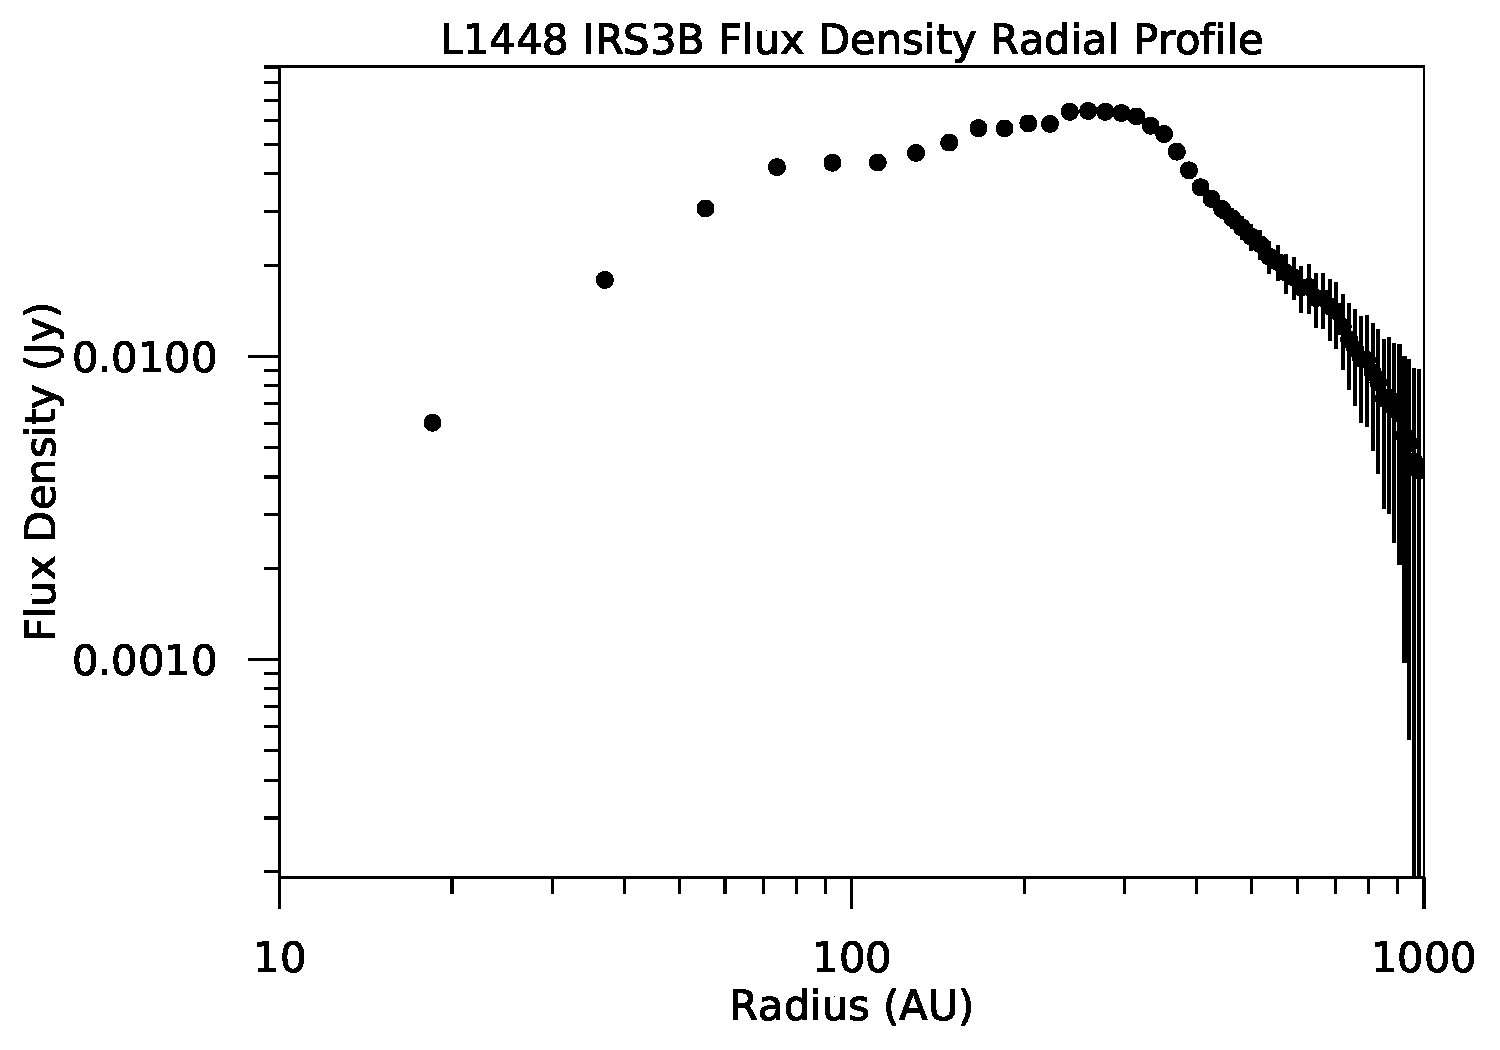
\includegraphics[width=0.48\textwidth]{img/L1448N-dgr-linear-intensity-c17o_cont.eps}
\includegraphics[width=0.48\textwidth]{img/L1448N-dgr-loglog-c17o_cont.eps}
\end{center}   
\caption{\textbf{Left:} A comparison plot between the dust surface density (blue) and the gas surface density (green) as a function of radius throughout the disk. The dust peaks at a local minima between two local maxima of the gas surface density, indicating a dust trapping mechanism.}\label{fig:gdr}
\end{figure}

%discuss peak PV %This actually looks pretty good! The green line has slope of -0.5 right? Can you plot a slope of -1 just for reference starting at around 100 AU? How does the M=0.8 M_sun match up with the fit from flared_model? At R< 30 AU, I think things flatten out because inward of that radius I don't think the emission was getting any closer to the protostar for whatever reason. One of the assumptions that this type of graph maps is that the emission is compact and the position has a direct relationship with the velocity of the keplerian gas. This assumption is not exactly true, especially when a disk is as well-resolved as L1448 IRS3B is. So, that is partly why the points start to drop below the line because the centroid is moving out pretty fast. I think the Keplerian radius is under estimated from plots like these. 

%#%#%#%#%#%#%#%#%#%#%#%#%#%#%#%#%#%#%#%#%#%#%#%#%#%#%#
%#%# Future Work %#%#
%#%#%#%#%#%#%#%#%#%#%#%#%#%#%#%#%#%#%#%#%#%#%#%#%#%#%#
\subsection{Future Work}
\subsubsection*{Dust Trapping}
Analyzing the radial profile of the GDR for IRS3B, the dust peaks at a local minima between two local maxima of the gas surface density, indicating a dust trapping mechanism. This is further supported as \citet{2015MNRAS.451..974D} showed spiral arms can be caused by pressure bumps within the disk, where the small grains follow with the gaseous material and the larger grains settle into the local minima between pressure walls. 

\subsubsection*{Feeding GI}
It is thought that massive disks are built up through accreting material from the collapsing protostellar envelope, drawing a possible correlation between an infalling envelope with the turbulent disk which we can test \citep[e.g.][]{2010ApJ...708.1585K,2010ApJ...725.1485O}. However, to understand the formation and sustainment of these gravitationally unstable disks, we need to directly connect such systems to their surrounding envelopes. Theories suggest multiple formation can occur via turbulent core fragmentation \citep[e.g.][]{2018ApJ...856..147O} and/or disk fragmentation \citep{2010ApJ...710.1375K} and while ALMA is able to detect these systems \citep[see][]{2012MNRAS.420L..53O}, it has yet to be vigorously tested.

%#%#%#%#%#%#%#%#%#%#%#%#%#%#%#%#%#%#%#%#%#%#%#%#%#%#%#
%#%# Conclusion %#%#
%#%#%#%#%#%#%#%#%#%#%#%#%#%#%#%#%#%#%#%#%#%#%#%#%#%#%#
\section{Summary}
We present the highest spatial and spectral resolution observations to date of L1448 IRS3B for continuum and spectral lines. We resolved the kinematic structures surrounding the source and compared with radiative transfer models tracing disk closely the gas and dust components. The inclusion of the tertiary source of the triple system, coupled with the spiral arms, is indicative of fragmentation pathways through gravitational instability. The main results of our analysis can be summarized as followed:
\begin{enumerate}
    \item Observed L1448 IRS3B, a young, nearby, triple protostellar system in the Perseus Molecular Cloud. We targeted Band 7 (879~\micron) with a plethora of lines and observed \lcso\space and \lhtcn\space emission as kinematic tracers of the disks surrounding IRS3B and IRS3A, respectively.
    \item We resolved the spirals of IRS3B and marginally resolved the spirals of IRS3A and observed IRS3B-c, the tertiary, to be embedded within one of the spiral arms.
    \item Through analyzing the continuum observations of IRS3B and making the assumptions outlined in Section~\ref{sec:surfden}, we estimate the disk surrounding IRS3B is \ab0.64\solm\space with about 0.09\solm\space mass in the tertiary companion, IRS3B-c. IRS3A has a compact, low mass disk of \ab0.08\solm.
    \item Found that the \cso, \htcop,and \htcn\space emission are indicative of a Keplerian disk with a central mass of 1.4 and 1.1\solm, for IRS3A and IRS3B respectively.
    \item The high spatial and spectral resolution observations allow azimuthally integrated radial profiles to be made to analyze the gravitational stability as a function of radius. We find the disk is gravitationally unstable (Toomre Q $<$ 1) for radii $>$ 120 AU.
    \item We further validate our findings of a massive gravitationally unstable disk surrounding the triple system L1448 IRS3B with robust radiative transfer modeling (Section~\ref{sec:surfden}) using both the continuum and kinematic capabilities of our code.
\end{enumerate}

%#%#%#%#%#%#%#%#%#%#%#%#%#%#%#%#%#%#%#%#%#%#%#%#%#%#%#
%#%# References %#%#
%#%#%#%#%#%#%#%#%#%#%#%#%#%#%#%#%#%#%#%#%#%#%#%#%#%#%#
\begin{small}
\bibliographystyle{apj}
\bibliography{ms}
\end{small}
\clearpage
%#%#%#%#%#%#%#%#%#%#%#%#%#%#%#%#%#%#%#%#%#%#%#%#%#%#%#
%#%# Affiliations %#%#
%#%#%#%#%#%#%#%#%#%#%#%#%#%#%#%#%#%#%#%#%#%#%#%#%#%#%#
% \section*{Affiliations}
% \begin{enumerate}
% \item Homer L. Dodge Department of Physics and Astronomy, University of Oklahoma, 440 W. Brooks Street, Norman, OK 73019, USA
% \item National Radio Astronomy Observatory, P.O. Box O, Socorro, NM 87801
% \item Department of Astronomy, University of Illinois, Urbana, IL 61801
% \item Department of Astronomy, University of Virginia, Charlottesville, VA 22903
% \item Harvard-Smithsonian Center for Astrophysics, 60 Garden St, MS 78, Cambridge, MA 02138
% \item Department of Physics, State University of New York Fredonia, Fredonia, New York 14063, USA
% \item Harvard-Smithsonian Center for Astrophysics, 60 Garden St, MS 78, Cambridge, MA 02138
% \item Department of Astronomy, University of Illinois, Urbana, IL 61801
% \item University of Arizona, Steward Observatory, Tucson, AZ 85721
% \item Center for Astrophysics and Space Sciences, University of California, San Diego, CA 92093
% \item Department of Astronomy, University of Illinois, Urbana, IL 61801
% \item Departamento de Astronom\'ia, Universidad de Chile, Camino El Observatorio 1515, Las Condes, Santiago, Chile
% \end{enumerate}
%#%#%#%#%#%#%#%#%#%#%#%#%#%#%#%#%#%#%#%#%#%#%#%#%#%#%#
%#%# Acknowledgements %#%#
%#%#%#%#%#%#%#%#%#%#%#%#%#%#%#%#%#%#%#%#%#%#%#%#%#%#%#
\section*{Ackowledgements}
This paper makes use of the following ALMA data: 2016.1.01520.S. ALMA is a partnership of ESO (representing its member states), NSF (USA) and NINS (Japan), together with NRC (Canada), MOST and ASIAA (Taiwan), and KASI (Republic of Korea), in cooperation with the Republic of Chile.  The Joint ALMA Observatory is operated by ESO, AUI/NRAO and NAOJ. The National Radio Astronomy Observatory is a facility of the National Science Foundation operated under cooperative agreement by Associated Universities, Inc. [Some of] The computing for this project was performed at the OU Supercomputing Center for Education \& Research (OSCER) at the University of Oklahoma (OU). This research has made use of NASA's Astrophysics Data System.
\newpage
%#%#%#%#%#%#%#%#%#%#%#%#%#%#%#%#%#%#%#%#%#%#%#%#%#%#%#
%#%# Ancillary %#%#
%#%#%#%#%#%#%#%#%#%#%#%#%#%#%#%#%#%#%#%#%#%#%#%#%#%#%#
\section{Ancillary}\label{sec:anc}
\explain{Cut IRS33B-ab and merged with IRS3B for clarity.}
\begin{deluxetable}{ccccccc}
\tablewidth{0pt}
%\rotate
\tabletypesize{\scriptsize}
\tablecaption{PV Diagram Fitting}
\tablehead{
  \colhead{Source} & \colhead{Center RA} & \colhead{Center Dec} & \colhead{Inclination} & \colhead{Position Angle} & \colhead{Stellar Mass} & \colhead{Velocity} \\
  & \colhead{(\arcsec)} & \colhead{(\arcsec)} & \colhead{(\deg)} & \colhead{(\deg)} & \colhead{(\solm)} & \colhead{(km~s$^{-1}$)}\\
}
\startdata
IRS3B    & 03$^{h}$25$^{m}$36.317$^{s}$ & 30\deg45\arcmin15\farcs005 & 45 & 29 & 1.15$^{+0.09}_{-0.09}$ & 4.8\\ %& 0.64\\
IRS3B-c  & 03$^{h}$25$^{m}$36.382$^{s}$ & 30\deg45\arcmin14\farcs715 & - & - & $<$0.2\tablenotemark{a} & - \\%& -\\
IRS3A    & 03$^{h}$25$^{m}$36.502$^{s}$ & 30\deg45\arcmin21\farcs859 & 69 & 125 & 1.4\tablenotemark{b}& 5.4\\ %&  0.06 \\
\enddata
\tablecomments{Summary of PV diagram stellar parameter estimates with 3-$\sigma$\space confidence interval of the best fit walkers generated from emcee. The inclination and position angle estimates are provided by 2-D Gaussian fitting of the uv-truncated data and is further confirmed with the PV diagram analysis.}
\tablenotetext{a}{\replaced{IRS3B-c, was only marginally constrained through the PV diagram analysis. The source dust component, while optically thick, is estimated to be no more than 0.2~\solm\space to be consistent with the data.}{The upper limit for IRS3B-c of $<$0.2~\msun\space is derived from its apparent lack of significant influence on the disk kinematics within its immediate proximity. Furthermore, we estimate from the dust emission that the mass of the gas and dust clum surrounding the protostar is \ab0.07~\msun. So the combined mass of the clump and protostar must be $<$0.2~\msun.} \deleted{Through analyzing the \cso\space PV diagram emission and considering the gravitational potential of IRS3B-ab, we estimate the upper mass limit of the tertiary source. }Figure~\ref{fig:l1448irs3b_c17o_pv_tert} shows the mass limit estimates of the tertiary of the source, with emission outside of the dotted lines indicating additional mass if perturbing the disk.}
\tablenotetext{b}{IRS3A, was marginally resolved and no sufficient numeric fits could be achieved with simple PV-diagram fitting. These estimates are provided by fitting the curve by eye and are not designated to be the final results and simply provide further constraints for the priors for the more rigorous kinematic modeling.}
\end{deluxetable}\label{table:pvtable}

\begin{deluxetable}{cccccccc}
\tablewidth{0pt}
%\rotate
\tabletypesize{\scriptsize}
\tablecaption{Continuum and Spectral Line Data}
\tablehead{
  \colhead{} & \colhead{MFS Continuum\tablenotemark{a}} & \colhead{\co} & \colhead{\sio\tablenotemark{b}} & \colhead{\htcn/\sot\tablenotemark{c}} & \colhead{\htcop} & \colhead{\cso}  & \colhead{335.5GHz Continuum} \\
}
\startdata
% Spectral Window     & -         & 0          & 1             & 2           & 3          & 4           & 5           \\
 Rest. Freq. (GHz)   & 341.0     & 346.0             & 347.000030579  & 345.339756     & 346.998347     & 337.061104      & 335.5       \\
 Center Freq. (GHz)  & 341.0     & 346.778059        & 347.2698586    & 345.3520738    & 347.010582     & 337.0730133     & 335.4708304 \\
 Chan. Width (km/s)  & 2747.96   & 0.212             & \replaced{0.053}{0.210}          & 0.053          & 0.053          & 0.054           & 0.873       \\
 Num. Chan.          & 1         & 1920              & 1920           & 1920           & 1920           & 3840            & 1920        \\
 RMS/chan. (mJy)     & 0.069     & 4.0               & 0.5            & 4.5            & 4.5            & 3.7             & -           \\
 Integr. (Jy) IRS3B\tablenotemark{d}  & 1.5       & 512.7,809.8\tablenotemark{e} & 7.8, 3.5\tablenotemark{e} & 0.2, 0.1\tablenotemark{e} & 2.6, 4.1\tablenotemark{e}& 2.9, 3.2\tablenotemark{e} & -           \\
 Integr. (Jy) IRS3A\tablenotemark{d}  & 0.2       & 3.16,67.6\tablenotemark{e}   & 0,0 \tablenotemark{e}     & 2.3, 2.7\tablenotemark{e} & 0.2, 0.4\tablenotemark{e} & 0.1, 0.1\tablenotemark{e} & -           \\
 Synth. Beam\tablenotemark{f}         & \contbeam & \cobeam           & \siobeam       & \htcnbeam      & 0\farcs21$\times$0\farcs13     & \csobeam        & \tttfbeam   \\
 Briggs Robust       & 0.5       & 0.5               & 0.5            & 0.5            & 0.5            & 0.5             & -           \\
 Taper (k$\lambda$)  & -         & -                 & -              & 1000           & 1500            & 1500            & -           \\
\enddata 
\tablecomments{The setup of the correlator for the observations}
\tablenotetext{a}{Multi-Frequency Synthesis (MFS) utilizing the extracted emission from line free spectral channels}
\tablenotetext{b}{\sio\space was tuned incorrectly for the C40-6 observations.}
\tablenotetext{c}{The \htcn\space line is blended with the \sot\space line (345.3385377~GHz) and have a velocity separation of \ab1.06~km~s$^{-1}$.}
\tablenotetext{d}{The integrated flux density for the source, measured by integrated the full emission whose origin is the source. In the case of continuum emission, this is given in \textit{Jy}; in the case of molecular line emission this is given in \textit{Jy~km~s$^{-1}$}.}
\tablenotetext{e}{The molecular line emission is given as the total integrated flux (Jy~km~s$^{-1}$) for the blue and red-Doppler shifted emission, denote blue, red, respectively.}
\tablenotetext{f}{The synthesized beam size is provided from the \textit{clean} task for the molecular lines (or continuum for the MFS column) using the briggs robust weighing parameter of 0.5 during image reconstruction.}
\end{deluxetable}\label{table:obssummary2}
% The combined observations achieved 0.069~mJy~beam$^{-1}$ (beam: \contbeam) continuum sensitivity, 4~mJy~beam$^{-1}$~channel$^{-1}$~(width: 0.423~km~s$^{-1}$, beam: \cobeam) for \co, 3.7~mJy~beam$^{-1}$~channel$^{-1}$~(width: 0.109~km~s$^{-1}$, beam: \csobeam) for \cso, 4.5~mJy~beam$^{-1}$~channel$^{-1}$~(width: 0.106~km~s$^{-1}$, beam: \htcnbeam) for \htcn/\sot, 4.5~mJy~beam$^{-1}$~channel$^{-1}$~(width: 0.105~km~s$^{-1}$, beam: \htcopbeam) for \htcop, and 0.5~mJy~beam$^{-1}$~channel$^{-1}$~(width: 0.422~km~s$^{-1}$, beam: \siobeam) for \sio.
\movetabledown=2in
\begin{splitdeluxetable}{cccccccBccccccccc}
\rotate
\tablewidth{0pt}
%\rotate
\tabletypesize{\scriptsize}
\tablecaption{Source Properties}
\tablehead{
 \colhead{Source} & \colhead{RA}      & \colhead{Dec}     & \colhead{Inc.\tablenotemark{a}} & \colhead{P.A.\tablenotemark{b}}  & \colhead{Outflow?} & \colhead{V$_{sys}$}      & \colhead{L$_{bol}$}  & \colhead{M$_{dust}$}  & \colhead{FWHM$_{Dust}$\tablenotemark{c} Major Axis} & \colhead{FWHM$_{Dust}$\tablenotemark{c} Minor Axis} & \colhead{FWHM$_{Gas}$\tablenotemark{c} Major Axis} & \colhead{FWHM$_{Gas}$\tablenotemark{c} Minor Axis}  & \colhead{$<$T$_{0}>$} & \colhead{$<$Optical Depth$>$} \\
                  & \colhead{(J2000)} & \colhead{(J2000)} & \colhead{(\deg)}                & \colhead{(\deg)}                 &                    & \colhead{(km~s$^{-1}$)}  & \colhead{(\lsun)}    & \colhead{(\solm)}                             & \colhead{(\arcsec, au)}                 & \colhead{(\arcsec, au)} & \colhead{(\arcsec, au)}                 & \colhead{(\arcsec, au)}   & \colhead{(K)} & & \\
}
\startdata
 IRS3B-ab & 03:25:36.317 & 30:45:15.005 & 45 & 28  & Joint & 4.75 & 13.0\tablenotemark{e}  & 0.29 & 1.73$\pm$0.05, 498$\pm$14 & 1.22$\pm$0.04, 351$\pm$12 & 2.38$\pm$0.09, 685$\pm$26 & 2.25$\pm$0.08, 648$\pm$23 & 40 & 0.34 \\
 IRS3B-c  & 03:25:36.382 & 30:45:14.715 & 27 & 21  & Yes   & 4.75 & -\tablenotemark{d}     & 0.07 & 0.28$\pm$0.05, 81$\pm$14  & 0.25$\pm$0.04, 72$\pm$12  & -                         & -                         & 55 & 2.14 \\
 IRS3A    & 03:25:36.502 & 30:45:21.859 & 69 & 133 & No    & 5.2  & 14.4\tablenotemark{e}  & 0.04 & 0.70$\pm$0.02, 202$\pm$6  & 0.25$\pm$0.01, 72$\pm$3   & 0.52$\pm$0.08, 150$\pm$23 & 0.42$\pm$0.07, 121$\pm$20 & 51 & 0.57 \\
\enddata
\tablecomments{Summary of the empirical parameters based from the observations of the system. The sizes were derived from a 2-D Gaussian fit to the continuum and moment 0 emission maps, directly to the visibilities. IRS3B-c is blended with the underlying disk continuum and estimates here are extracted from a 2-D gaussian fit with a zero-level offset to preserve the underlying disk flux and is discussed in Appendix~\ref{sec:tertsub}.}
\tablenotetext{a}{Inclination is defined such that 0\deg\space is a face-on disk.}
\tablenotetext{b}{Position angle is defined such that at 0\deg, the major axis of the disk is aligned North and the angle corresponds to East-of-North.}
\tablenotetext{c}{The circumstellar disks surround IRS3B and IRS3A are ellipsoidal in the dust continuum and molecular line emission.}
\tablenotetext{d}{The bolometric luminosity is not known at this time.}
\tablenotetext{e}{The bolometric luminosity is scaled to a distance of 288~pc\space from \citet{2016ApJ...818...73T}.}
\end{splitdeluxetable}\label{table:obssummary3}

\begin{deluxetable}{cccccccccccc}
\rotate
\tablewidth{0pt}
%\rotate
\tabletypesize{\scriptsize}
\tablecaption{Kinematic \pdspy Modeling}
\tablehead{
  \colhead{Source} & \colhead{RA Offset} & \colhead{Dec Offset} & \colhead{Inc.} & \colhead{P.A.} & \colhead{M$_{*}$} & \colhead{M$_{gas}$\tablenotemark{a}} &\colhead{R$_{disk}$} & \colhead{V$_{sys}$}& \colhead{Turbulence}& \colhead{Surface Density Index $\gamma$} & \colhead{T$_{0}$}\\
  & \colhead{(\arcsec)} & \colhead{(\arcsec)} & \colhead{(\deg)} & \colhead{(\deg)} & \colhead{(\solm)} & \colhead{(\solm)}& \colhead{(au)} & \colhead{(km~s$^{-1}$)}& \colhead{(km~s$^{-1}$)}& & \colhead{(K)}  \\
}
\startdata
IRS3B  & $0.031^{+0.019}_{-0.011}$ & $0.025^{+0.020}_{-0.015}$ & $66.0^{+ 3.0}_{- 4.6} $ & $26.7^{+  1.8}_{-  2.9} $ & $1.19^{+0.13}_{-0.07}$ & $0.079^{+0.021}_{-0.016}$ & $299.0^{+ 24.9}_{- 47.6}$ & $4.880^{+0.110}_{-0.090}$ & $0.012^{+ 0.005}_{- 0.003}$ & $  1.2^{+  0.1}_{-  0.1}$&$   50^{+    3}_{-    5}$\\
IRS3A  & $0.034^{+0.003}_{-0.003}$ & $0.015^{+0.003}_{-0.003}$ & $69.5^{0.38}_{0.37} $  & $122.4^{1.4}_{1.4}$ & $1.51^{+0.06}_{-0.07}$ & $6.3^{+1.6}_{-1.3}x10^{-6}$ & $ 39.9^{+  2.4}_{-  1.4}$ & $5.288^{+0.090}_{-0.084}$ & $0.015^{+ 0.06}_{-0.009}$ & $0.4^{+0.2}_{-0.1}$ & $163^{+9}_{-8}$ \\
% /home/reynolds/local/PDSPY_models/L1448IRS3A/h13cn/localruns/
% /home/reynolds/lovell1/c17o
\enddata
\tablecomments{Summary of kinematic model parameters. The RA and DEC offsets of the \pdspy modeling are defined from the central positions given in PV Analysis, Table~\ref{table:pvtable}. The errors presented are the 3-$\sigma$\space confidence intervals of the best fit walkers generated from \textit{emcee}.}
\tablenotetext{a}{\added{The reported values of M$_{gas}$\space depend on the assumed abundance for each of the molecules. For the IRS3B source, we used the \cso\space emission, which has an assumed abundance of $2\times10^{-7}$ relative to H$_{2}$, while for the IRS3A source we used the \htcn\space emission which has an assumed abundance of $2.9\times10^{-11}$ relative to H$_{2}$.}}
\end{deluxetable}\label{table:pdspykinematic}

% /net/ryle/myhome1/reynolds/PDSPY_models/oscer/wide/h13cn
% ~/jansky1/c17o
% irs3bcont
% irs3acont

\input{tables/continuumtable.tex}

\subsection{Molecular Line Emission}
The \co\space moment map (Appendix~\ref{sec:momentmaps}) shows clear signs of a collimated outflow originating from a region near the inner binary of IRS3B. Emission from IRS3A show indications of wide angled, low velocity outflows orthogonal to the outflows in IRS3B. The implications are discussed later. In Appendix~\ref{sec:momentmaps}, we show \sio, an indicator shocked gas fronts. These locations correspond to the collisions of the outflows indicated by \co\space with the surrounding gas. These regions are very detailed structures near launch location and show regions of large, slow gaseous clumps that interact with the outflows, producing massive (d\ab760 AU) lobes.

\clearpage
\subsection*{Moment Maps}\label{sec:momentmaps}
\begin{figure}[H]
\begin{center}
\includegraphics[width=\textwidth]{img/cont_fit.eps}
\end{center}
\caption{IRS3B continuum modeling graphical results of the MCMC fit. The axes represent the difference parameters and the plot demonstrates both the covariance of the parameters and the convergence. Both the blue dots and lines indicate the median fit for each of the parameters and show the respective covariance fit against a histogram of the same.}\label{fig:stairstep_cont}
\end{figure}
\newpage
\begin{figure}[H]
\begin{center}
\includegraphics[width=\textwidth]{img/c17o_fit.eps}
\end{center}
\caption{IRS3B \cso\space kinematic modeling grahical result. Similar to the continuum model fit prior, this plot summarizes the convergence and covariance of the modelled parameters. Both the blue dots and lines indicate the median fit for each of the parameters and show the respective covariance fit against a histogram of the same.}\label{fig:stairstep_c17o}
\end{figure}
\newpage
\begin{figure}[H]
   \begin{center}
   \includegraphics[width=\textwidth]{img/L1448IRS3B_12CO_image_binned_clean__binnedMoments.eps} % co
   \includegraphics[width=\textwidth]{img/L1448IRS3B_SiO_image_taper1500k__totalMoments.eps}
   \end{center}
   \vspace{-0.25cm}\caption{ The Moment 0 map (integrated intensity) of the respective lines, overlaid the continuum (grayscale) image from Figure~\ref{fig:contimage}. 
   \textbf{Top (A):} \co\space detailing in exquisite detail the location and collimated of the IRS3B outflows. The central outflow from IRS3B extends 10\arcsec\space(2900 AU) from launch location on either side. Contours start at 10(8)~$\sigma$ and iterate by 8(8)~$\sigma$ for the red(blue). respectively. 
   \textbf{Bottom (B):} \sio\space locations of shocked gas fronts. Contours start at 3(3)~$\sigma$ and iterate by 5(5)~$\sigma$ for the red(blue).}\label{fig:momentmap}
\end{figure}

%#%#%#%#%#%#%#%#%#%#%#%#%#%#%#%#%#%#%#%#%#%#%#%#%#%#%#
%#%# Tertiary %#%#
%#%#%#%#%#%#%#%#%#%#%#%#%#%#%#%#%#%#%#%#%#%#%#%#%#%#%#
\subsection{Tertiary Subtraction and Source Deprojection}
In order to analyze the circumstellar dust disk, independent of the tertiary, the bright source embedded within the binary spiral arm of the disk needs to be removed. This tertiary source, being the brightest source of this system, masks the underlying flux of the disk and contaminates the analysis of the disk structure. By removing this source, we independently study the disk and the tertiary source in order to characterize their properties separately (Figure~\ref{fig:subclump}).

\begin{figure}[H]
  \begin{minipage}[c]{\textwidth}
   \includegraphics[width=0.48\textwidth]{img/Per33_ALMA_cont_robust05_subclumpsplitMoments.eps} % co
   \includegraphics[width=0.48\textwidth]{img/L1448IRS3B_cont_ms_apselfcal_concat_subclump_deprojsplitMoments.eps} % co
  \end{minipage}
   \caption{Continuum (879~\micron) images of IRS3B. 
   \textbf{A Top Left:} IRS3B with the tertiary clump removed for analysis. The tertiary model was constructed using a 2D Gaussian with a zero-level offset in order to properly restore the underlying disk emission without introducing additional features. This residual image was then used for further analysis and modeling via RADMC-3D.} \label{fig:subclump}
\end{figure}
% work on this
In order to remove the tertiary source, we fit two Gaussians with a zero-level offset to the position of the source using the \textit{imfit} task in casa. The offset serves to preserve the emission from the underlying disk emission. We also restricted the imfit task to a 0\farcs8$\times$0\farcs7\space ellipse around the source as to not extend the fit into the surrounding emissions from the spiral arms. With these parameters generated from the imfit task, we then constructed a model image of the tertiary that was then used to construct a model visibility dataset via the Fourier transform and set the flux density of the measurement with the task \textit{setjy}. This populates the model column of a CASA measurement set with the source visibility data, which we then use the task \textit{uvsub} to subtract this model with the data, producing the residual visibilities without the tertiary. A tertiary subtracted image is generated from this residual dataset and shown in Figure~\ref{fig:subclump}.

To determine the position angle and inclination of the disk, we fit the semi-major and semi-minor axis of the disk with a 2-D Gaussian provided by the \textit{imfit} routine. In order to fit the general shape of the disk and not fit the shape of the spiral arms, we smooth (taper the UV visibilities at 350 k$\lambda$) to recover the spiral arm flux but unresolve the underlying structure and provide a more appropriate image for single 2D Gaussian fitting. For the IRS3B source, we restrict the fit to a 2\arcsec$\times$2\arcsec\space region centered on IRS3B-a which appears to be the more centrally located protostar. 

From this fit, we recovered the inclination and position angle of the disks. The protostellar disk of IRS3B had a semi-major axis and semi-minor axis of 1\farcs84\space and 1\farcs29\space (\ab540 AU $\times$\space \ab377 AU), respectively. This corresponds to an inclination angle of 45.8\deg\space assuming the disk is axially symmetric. We estimate the uncertainty to be as much as 25\% \space by fitting each side of image split by the semi-major axis separately. The position angle of the disk corresponds to 29.1\deg\space East-of-North.

The protostellar disk of IRS3A had a semi-major axis and semi-minor axis of 0\farcs68\space and 0\farcs28\space(\ab200 AU $\times$\space \ab82 AU), respectively. This corresponds to an inclination angle of 65.9\deg assuming the disk is axially symmetric. The position angle of the disk corresponds to 132.5\deg\space East-of-North.

%#%#%#%#%#%#%#%#%#%#
%#%# End of doc %#%#
%#%#%#%#%#%#%#%#%#%#

\end{document}
